\documentclass[11pt, oneside]{article}  
\usepackage[margin=0.5in]{geometry} % Margins
\usepackage[ampersand]{easylist} % Bullets for lists
\usepackage[bottom]{footmisc}  % Glue footnotes to bottom
\usepackage{listings}
\usepackage{amsmath}
\usepackage{float}
\usepackage{array,mathtools}

\newcommand*{\carry}[1][1]{\overset{#1}}
\newcolumntype{B}[1]{r*{#1}{@{\,}r}}

\title{Homework 2\\UCLA-CS180-S18}
\author{Quentin Truong}


\begin{document}
\maketitle
\pagenumbering{arabic}


%========================================================
\section{Question 1}

Piazza says this question only requires the complete algorithm and proof of main lemma \newline

Proof of Main Lemma: \newline
All points within points\_sy\_strip fall within min\_dist from the center (by definition).
Therefore, the strip is 2 * min\_dist wide.
If we vertically divide this strip into four, then horizontally divide this strip every 1/2 min\_dist, we will have 4 squares per row.
Each square will have side length 1/2 min\_dist.
The maximum distance between two points within one square is 1/2 * min\_dist + 1/2 * min\_dist (l1\_distance).
Knowing that two points in one square could only ever be min\_dist away from each other (if they were closer, min\_dist would be that value, bc two points in one square always fall on the same side)
and because we are only interested in pairs of points whose distance is less than min\_dist, we can claim that there is only one point per square.
If a point lay on the top of a row 1 and the bottom of row 4 (row 4 is above row 1), they would be separated by min\_dist. 
There are 4 boxes per row and 4 total rows, therefore there are 16 boxes.
The pair of points cannot be in the same box, otherwise they would have been on the same side and we would have had a different min\_dist.
Therefore, the min\_dist is no farther away than 15 possible boxes.
Since each box has at most 1 point, we only need to check the next 15 points (sorted along the y coordinate).
The time complexity of this is O(nlogn) by master theorem (a = 2, b = 2, f(n) = n).

Algorithm: 
\begin{lstlisting}
function l1_distance (first, second):
    return abs(first.x - second.x) + abs(first.y - second.y)

function find_closest_pair_brute (points):
    min_dist = inf
    for (i = 0; i < points.size(); i++)
        for (j = i + 1; j < points.size(); j++)
            if (min_dist > l1_distance(points[i], points[j]))
                min_dist = l1_distance(points[i], points[j])
                min_pair = (points[i], points[j])
    return min_pair, min_dist

function find_closest_pair_strip (points_sy):
    min_dist = inf
    for (i = 0; i < points_sy.size(); i++)
        for (j = 1; j <= 15 AND i + j < points_sy.size(); j++)
            if (min_dist > l1_distance(points_sy[i], points_sy[i + j]))
                min_dist = l1_distance(points_sy[i], points_sy[i + j])
                min_pair = (points_sy[i], points_sy[i + j])
    return min_pair, min_dist

function find_closest_pair_l1_helper (points_sx, points_sy):
    if (points_sx.size() <= 3)
        return find_closest_pair_brute(points_sx)

    // O(n) by just copying stuff over in a good way
    left_points_sx, left_points_sy = left_half(points_sx, points_sy) 
    right_points_sx, right_points_sy = right_half(points_sx, points_sy)

    left_pair, left_dist = find_closest_pair_l1_helper(left_points_sx, left_points_sy)
    min_pair, min_dist = find_closest_pair_l1_helper(right_points_sx, right_points_sy)

    if left_dist < min_dist
        min_dist = left_dist
        min_pair = left_pair

    // O(n) to find points within min_dist of center
    points_sy_strip = get_middle_strip(points_sx, min_dist)
    strip_pair, strip_dist = find_closest_pair_strip(points_sy_strip, min_dist)

    if strip_pair < min_dist
        min_dist = strip_dist
        min_pair = strip_pair

    return min_pair, min_dist

function find_closest_pair_l1 (points):
    points_sx = sort_x(set_to_list(points))
    points_sy = sort_y(set_to_list(points))

    return find_closest_pair_l1_helper(points_sx, points_sy)
\end{lstlisting}

\clearpage
%========================================================

%========================================================
\section{Question 2}
We split the problem into two subproblems (a = 2), each of size n / 2 (b = 2), and merging their solutions requires at most a single traversal (f(n) = O(n)). From master theorem, the time complexity is O(nlogn).

\begin{lstlisting}
function find_majority_element(elements):
    if (elements.size() <= 2)
        if elements[0] == elements[elements.size() - 1]
            return elements.size(), elements[0]
        return 0, null

    left_elements, right_elements = split_in_half(elements)

    count_left, majority_element_left = find_majority_element(left_elements)
    count_right, majority_element_right = find_majority_element(right_elements)

    if majority_element_left == majority_element_right
        return count_left + count_right, majority_element_left
    else if majority_element_left != null
        for element in right_elements
            if element == majority_element_left
                count_left++
        if count_left > elements.size() / 2
            return count_left, majority_element_left
        else
            return 0, null
    else if majority_element_right != null
        for element in left_elements
            if element == majority_element_right
                count_right++
        if count_right > elements.size() / 2
            return count_right, majority_element_right
        else
            return 0, null
\end{lstlisting}

\clearpage
%========================================================

%========================================================
\section{Question 3}
\begin{figure}[ht]
\begin{center}
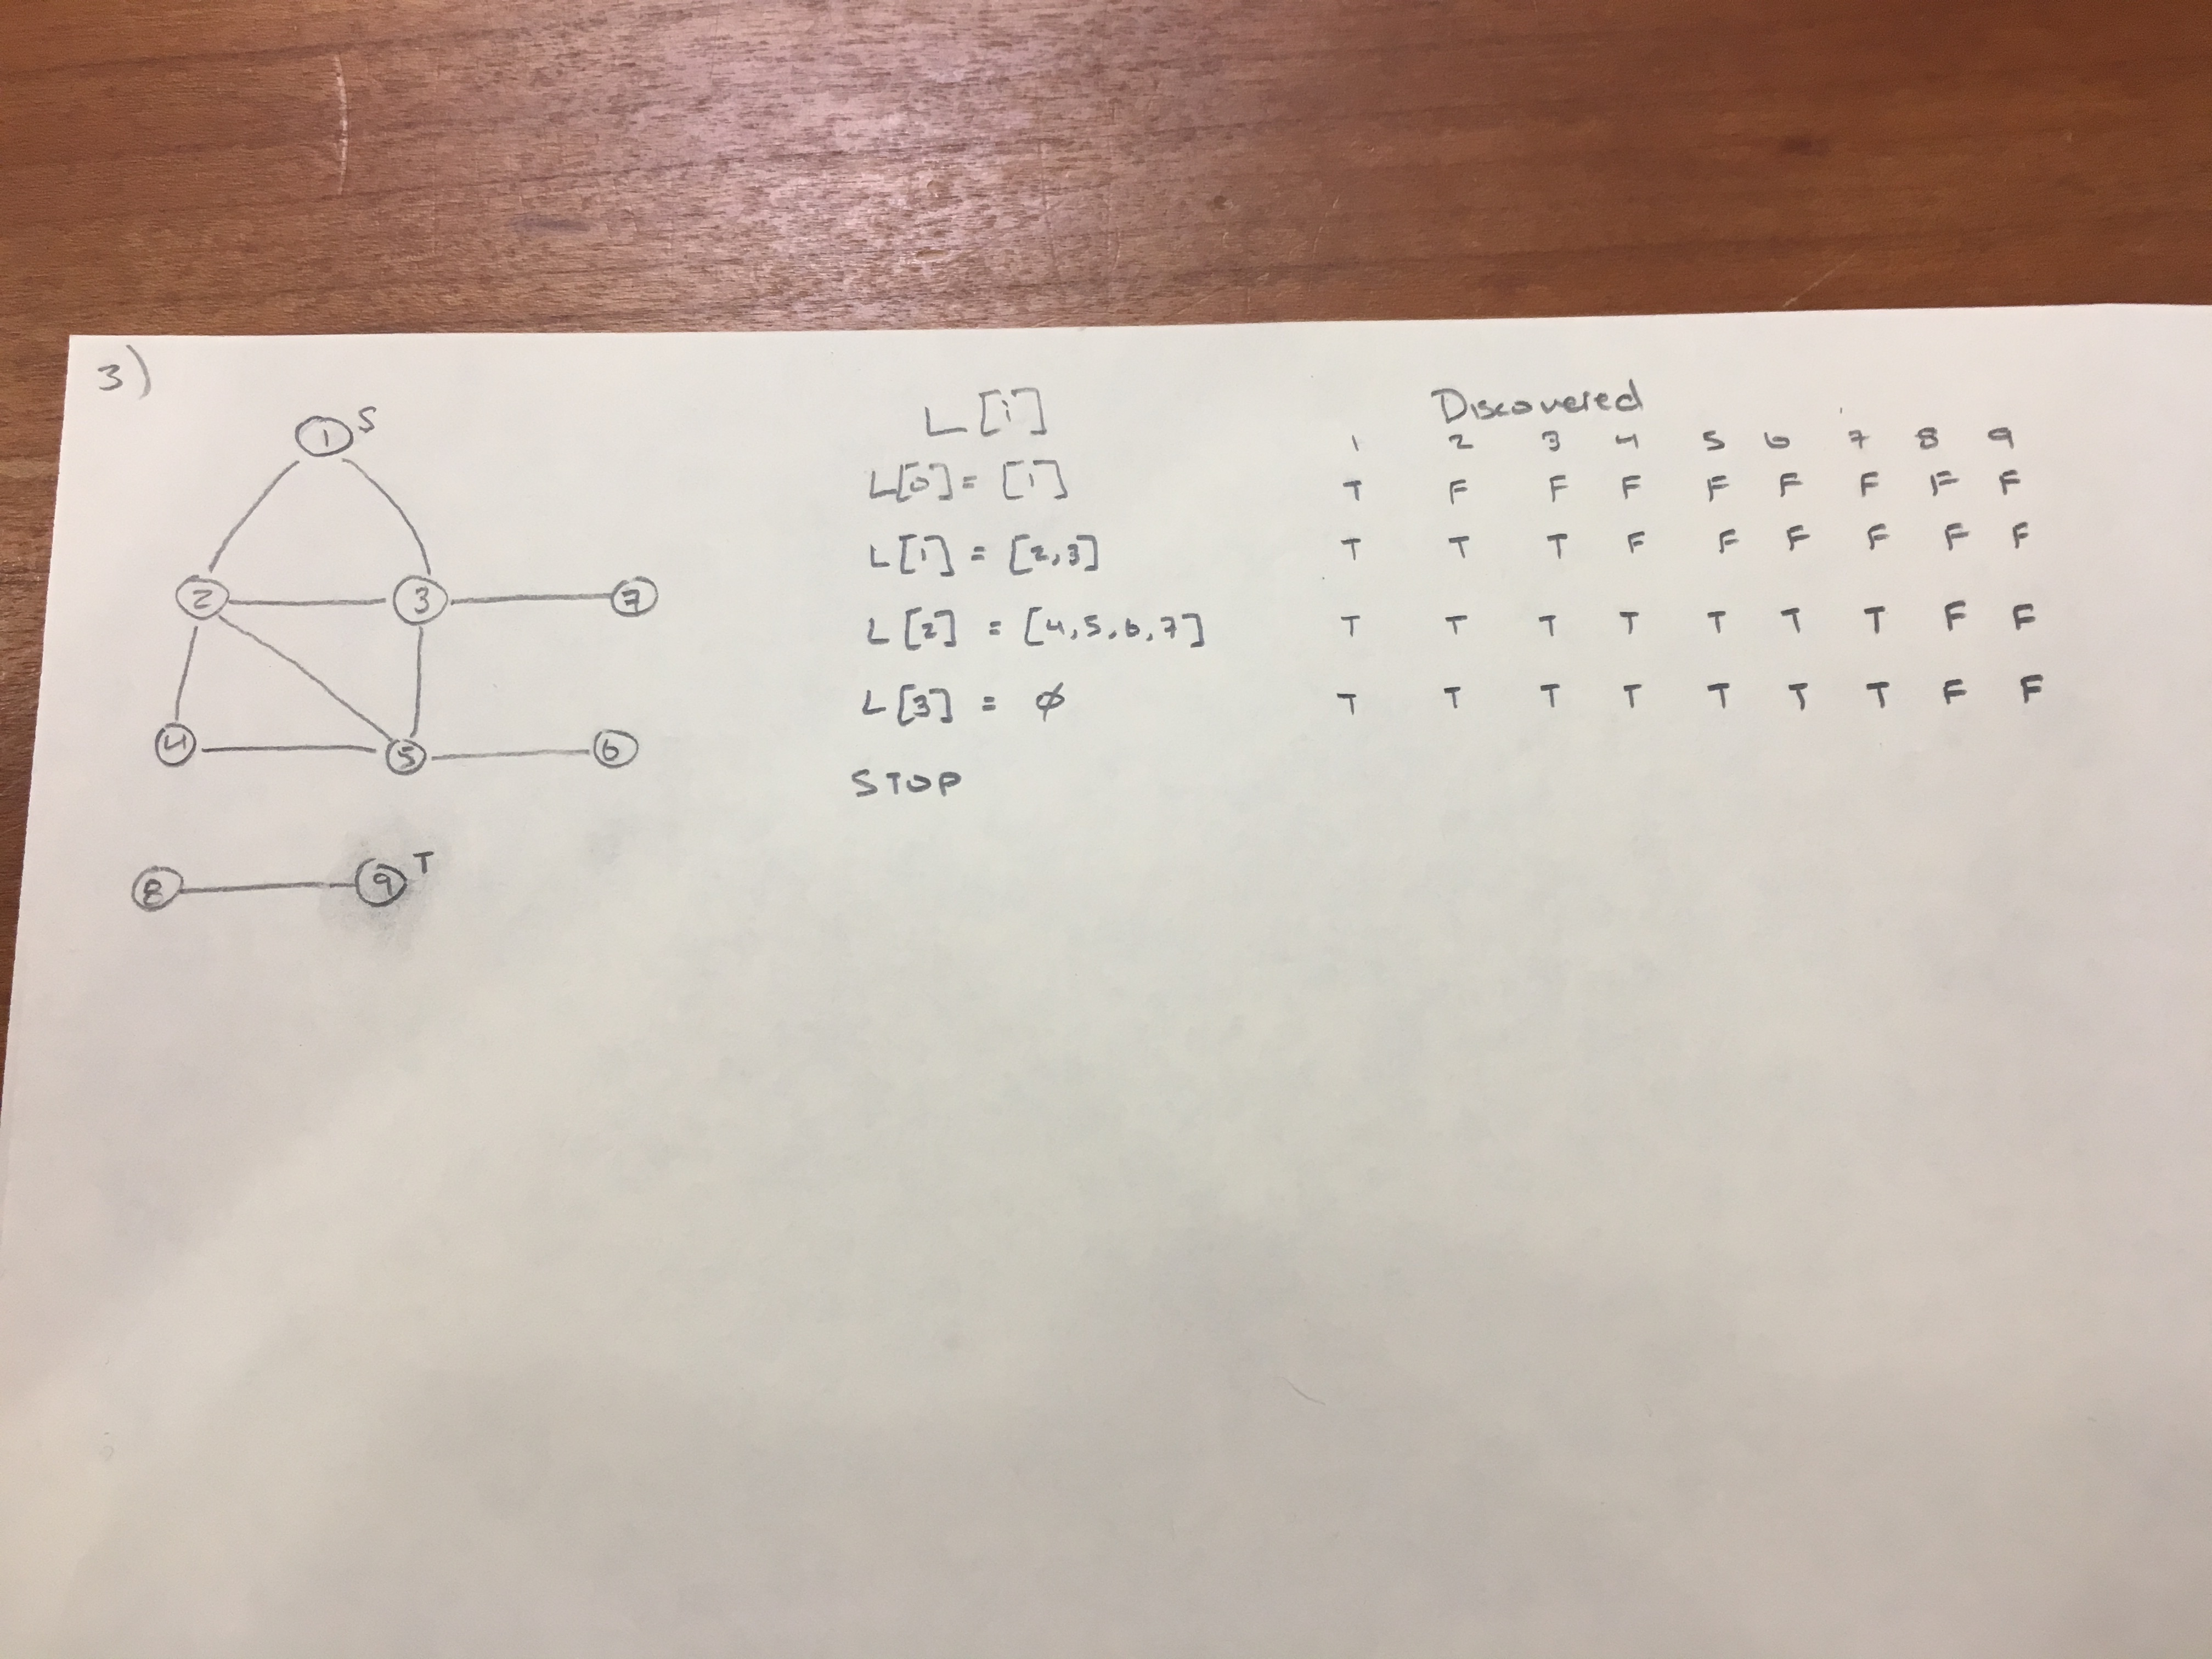
\includegraphics[width=\linewidth]{IMG_3161.JPG}
\end{center}
\end{figure}
\clearpage
%========================================================

%========================================================
\section{Question 4}

We traverse all vertices and check all their edges. Therefore, the time complexity is O(V * E).

\begin{lstlisting}
function has_triangle(graph, prev_layer, discovered)
    if (prev_layer.size() == 0)
        return false

    children = array of bool size n, init to false

    for curr in prev_layer
        for node in graph[curr]
            if discovered[node] == false
                next_layer.append(node)
                discovered[node] = true
                children[node] = true

    for curr in next_layer
        for node in graph[curr]
            if children[node] == true
                return true

    return has_triangle(graph, next_layer, discovered)

function has_triangle(graph)
    if (graph.size() == 0)
        return false

    discovered = array of bool of size n, init to false
    discovered[0] = true
    return has_triangle(graph, [0], discovered)
\end{lstlisting}

\clearpage
%========================================================

%========================================================
\section{Question 3.9 Kleinberg UNGRADED}
There’s a natural intuition that two nodes that are far apart in a communication network—separated by many hops—have a more tenuous connection than two nodes that are close together. There are a number of algorithmic results that are based to some extent on different ways of making this notion precise. Here’s one that involves the susceptibility of paths to the deletion of nodes. \newline
Suppose that an n-node undirected graph G = (V , E) contains two nodes s and t such that the distance between s and t is strictly greater than n/2. Show that there must exist some node v, not equal to either s or t, such that deleting v from G destroys all s-t paths. (In other words, the graph obtained from G by deleting v contains no path from s to t.) Give an algorithm with running time O(m + n) to find such a node v. \newline

For an n node, undirected graph, containing nodes s and t where their distance is strictly greater than n/2, there exist a node such that its deletion will remove any path from s to t. We know that the distance between s and t is  strictly greater than n/2, so at minimum, there are n/2 layers. If each layer has at least two nodes, then we have counted at least n/2 * 2 = n nodes; however, the graph only contains n nodes, and our count excludes node s and t. Therefore, there exist at least one layer without two nodes. This is valid for both odd and even n.\newline

Deleting this layer splits the original connected component into two connected components. This is clear because BFS has no other nodes to explore. Disconneted components have no path, by definition; therefore, deleting the layer containing only v will remove all paths from s to t.\newline

To find this node, we run BFS until we find the layer with only one node. We return this node. BFS is O(V + E). \newline


\clearpage
%========================================================

%========================================================
\section{Question 3.11 Kleinberg UNGRADED}
Design an algorithm that answers questions of this type: given a collection of trace data, the algorithm should decide whether a virus introduced at computer Ca at time x could have infected computer Cb by time y. The algorithm should run in time O(m + n). \newline

Create adjacency list using vector and list by traversing sequence. For triple (Ci, Cj, t), if t is in the inclusive range between x and y, create two nodes, (Ci, t) and (Cj, t). Connect those nodes bidirectionally. If there is another node involving computer Ci, create a directed path from the older to the newer. Do the same for Cj. \newline

Perform BFS from Ca. If Cb is discovered, then Cb could have been infected. This runs in O(m + n) because creating the adjacency list is O(m + n) and BFS is O(m + n). \newline

\clearpage
%========================================================

%========================================================
\section{Question 3.16 Dasgupta UNGRADED}
Suppose a CS curriculum consists of n courses, all of them mandatory. The prerequisite graph G has a node for each course, and an edge from course v to course w if and only if v is a prerequisite for w. Find an algorithm that works directly with this graph representation, and computes the minimum number of semesters necessary to complete the curriculum (assume that a student can take any number of courses in one semester). The running time of your algorithm should be linear. \newline

Create an array of the indegree count for each node. For each node curr, for each node neighbor of curr, increment its indegree count. \newline

Perform a modified BFS on the graph, counting the number of layers. Take the source layer to be any node with an indegree count of 0. For each node curr, for each node neighbor of curr, decrement its indegree count. If its new indegree count is 0, add it to the next layer. Repeat until no elements are added to the next layer. Return the number of required layers. The time complexity is O(m + n) because BFS is O(m + n). \newline

\clearpage
%========================================================

\end{document}